%\documentclass[12pt]{article}
%\usepackage[a4paper, margin=1in]{geometry} 
%\usepackage{graphicx} 
%\usepackage{hyperref}
%\usepackage{float}
%\usepackage{multicol}
%\usepackage{multirow}
%\usepackage{amsmath}
%\usepackage{amssymb}
%\usepackage[ruled]{algorithm2e}
%\usepackage[font=small, labelfont=bf]{caption}
%
%\begin{document}

%
% Aligning methods
%
\subsection{Aligning methods}
The progressive alignment method keeps combining two alignments until it produces the final alignment.

%
% Aligning methods for progressive alignment
%
\subsubsection*{Aligning methods for progressive alignment}
\begin{itemize}
\item Complete alignment
\item Pair-guided alignment
\item Conesus alignment
\item Profile alignment
\end{itemize}

%
% Complete alignment
%
\subsubsection*{Complete alignment}
It uses DP with a two-dimensional array to find gap positions between two alignments. \\

\noindent
The score of a cell at column $j$ and row $i$ can be calculated as: 
 \[
S(i,j)= \dfrac{1}{nm}\sum_{p \in \{p_1 \ldots p_n\}} \sum_{q \in \{q_1 \ldots q_m\}} R(\bar{s}_i^p,\bar{s}_j^q).
 \]

where $n$ and $m$ are the size of alignments, and $R(\cdot,\cdot)$ is a score function. \\

\noindent
\textbf{N.B.} Notice $R(-,-)$ is always 0.

%
% Example of complete alignment
%
\subsubsection*{Example of complete alignment}
Combine two alignments, $\mathcal{A}^p$ and $\mathcal{A}^q$ with a simple scoring scheme:  Match: 1, Mismatch: -1, and Gap penalty: 1.

\begin{table}[H]
\centering
\begin{tabular}{lllllll}
$\mathcal{A}^{p}$ & & \hspace{10em} & $\mathcal{A}^{q}$  & &  \\
 & $s^{p1}$: & \verb|GAT| &  &  & $s^{q1}$: & \verb|GT| \\
                        & $s^{p2}$: & \verb|G-T| &      &                         & $s^{q2}$: & \verb|A-| \\
                        &                          &     &      &                         & $s^{q3}$: & \verb|AT|
\end{tabular}
\end{table}

\textbf{DP table}

\begin{table}[H]
\centering
\begin{tabular}{ccccc}
  &                        & $s^{q1}$                           & G                     & T                     \\
  &                        & $s^{q2}$                           & A                     & -                     \\
  &                        & $s^{q3}$                          & A                     & T                     \\ \cline{3-5} 
$s^{p1}$ & \multicolumn{1}{c|}{$s^{p2}$} & \multicolumn{1}{c|}{0} & \multicolumn{1}{c|}{} & \multicolumn{1}{c|}{} \\ \cline{3-5} 
G & \multicolumn{1}{c|}{G} & \multicolumn{1}{c|}{}  & \multicolumn{1}{c|}{} & \multicolumn{1}{c|}{} \\ \cline{3-5} 
A & \multicolumn{1}{c|}{-} & \multicolumn{1}{c|}{}  & \multicolumn{1}{c|}{} & \multicolumn{1}{c|}{} \\ \cline{3-5} 
T & \multicolumn{1}{c|}{T} & \multicolumn{1}{c|}{}  & \multicolumn{1}{c|}{} & \multicolumn{1}{c|}{} \\ \cline{3-5} 
\end{tabular}
\end{table}

\textbf{Initialization} \\

$\begin{aligned}
S(0,1) &= \dfrac{1}{6}(-1 \times 6) &= -1 \\
S(0,2) &= -1 + \dfrac{1}{6}(-1 \times 4) &= -1.67 \\ \\
S(1,0) &= \dfrac{1}{6}(-1 \times 6) &= -1 \\
S(2,0) &= -1 + \dfrac{1}{6}(-1 \times 3) &= -1.5 \\
S(3,0) &= -1.5 + \dfrac{1}{6}(-1 \times 6) &= -2.5
\end{aligned} $
\bigskip \bigskip 

%
% NEWPAGE
%
\newpage

\textbf{Cell update: $S(1, 1)$} \\

$\begin{aligned}
S(1,1)^{(1)} & = -1 -1 = -2 \\
S(1,1)^{(2)} & = -1 -1 = -2 \\
S(1,1)^{(3)} & = \dfrac{1}{2\times3}((R(G,G)+R(G,A)+R(G,A))+(R(G,G)+R(G,A)+R(G,A))) \\
&=\dfrac{1}{6}((1-1-1)+(1-1-1))=-0.33
\end{aligned} $
\bigskip \bigskip 

\textbf{DP table after $S(1, 1)$ update}

\begin{table}[H]
\centering
\begin{tabular}{ccccc}
  &                        & $s^{q1}$                           & G                     & T                     \\
  &                        & $s^{q2}$                           & A                     & -                     \\
  &                        & $s^{q3}$                          & A                     & T                     \\ \cline{3-5} 
$s^{p1}$ & \multicolumn{1}{c|}{$s^{p2}$} & \multicolumn{1}{c|}{0} & \multicolumn{1}{c|}{-1} & \multicolumn{1}{c|}{-1.67} \\ \cline{3-5} 
G & \multicolumn{1}{c|}{G} & \multicolumn{1}{c|}{-1}  & \multicolumn{1}{c|}{-0.33} & \multicolumn{1}{c|}{} \\ \cline{3-5} 
A & \multicolumn{1}{c|}{-} & \multicolumn{1}{c|}{-1.5}  & \multicolumn{1}{c|}{} & \multicolumn{1}{c|}{} \\ \cline{3-5} 
T & \multicolumn{1}{c|}{T} & \multicolumn{1}{c|}{-2.5}  & \multicolumn{1}{c|}{} & \multicolumn{1}{c|}{} \\ \cline{3-5} 
\end{tabular}
\end{table}

%
% Pair-guided alignment
%
\subsubsection*{Pair-guided alignment}
Pair-guide alignment uses two sequences from two different alignments.

%
% Example of pair-guided alignment
%
\subsubsection*{Example of pair-guided alignment}
Combine two alignments, $\mathcal{A}^p$ and $\mathcal{A}^q$.

\begin{table}[H]
\centering
\begin{tabular}{lllllll}
$\mathcal{A}^{p}$ & & \hspace{10em} & $\mathcal{A}^{q}$  & &  \\
 & $s^{p1}$: & \verb|ACGG| &  &  & $s^{q1}$: & \verb|A-GTG| \\
                        & $s^{p2}$: & \verb|A-GG| &      &                         & $s^{q2}$: & \verb|ACGT-| \\
                        & $s^{p3}$: &  \verb|-CGG| &      &                         &  & 
\end{tabular}
\end{table}

\begin{figure}[H]
  \centering
      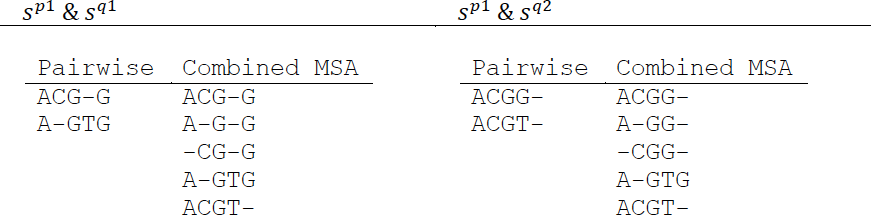
\includegraphics[width=0.9 \textwidth]{fig10/pair_guided_progress_alignment.png}
\end{figure}

%
% NEWPAGE
%
\newpage

%
% Exercise \thesection.2
%
\subsubsection*{Exercise \thesection.2}
Combine two alignments $\mathcal{A}^p$ and $\mathcal{A}^q$ by using the pair-guided approach.

\begin{table}[H]
\centering
\begin{tabular}{lllllll}
$\mathcal{A}^{p}$ & & \hspace{10em} & $\mathcal{A}^{q}$  & &  \\
 & $s^{p1}$: & \verb|TCG| &  &  & $s^{q1}$: & \verb|T-G| \\
                        & $s^{p2}$: & \verb|-CG| &      &                         & $s^{q2}$: & \verb|ACG| \\
                        & $s^{p3}$: &  \verb|T-C| &      &                         &  & 
\end{tabular}
\end{table}

\begin{enumerate}
\item Use the alignment between $s^{p3}$ and $s^{q2}$.

\begin{table}[H]
\centering
\begin{tabular}{ll}
 $s^{p3}$:& \verb|T-C-| \\
 $s^{q2}$:& \verb|-ACG|
\end{tabular}
\end{table}

\end{enumerate}
\bigskip 

%\end{document}
